% Standalone proof. Shared notation and prose conventions: analyses/README.md.
\documentclass[11pt,a4paper]{article}
\usepackage[T1]{fontenc}
\usepackage[utf8]{inputenc}
\usepackage{amsmath,amsthm}
\usepackage{newtxtext,newtxmath}
\usepackage[a4paper,margin=21mm,headheight=15pt]{geometry}
\usepackage{microtype,booktabs,array,tabularx,longtable}
\usepackage[table]{xcolor}
\usepackage{tikz,fancyhdr,enumitem,seqsplit}
\definecolor{Teal}{HTML}{176B70}
\definecolor{Ink}{HTML}{203443}
\definecolor{Pale}{HTML}{EDF5F5}
\definecolor{Line}{HTML}{C7D8DB}
\definecolor{Muted}{HTML}{536974}
\definecolor{Warm}{HTML}{F8F4EC}
\usepackage[colorlinks=true,linkcolor=Teal,urlcolor=Teal]{hyperref}
\color{Ink}
\newcommand{\blank}{\lambda}
\newcommand{\digits}{\{0,1\}}
\newcommand{\ph}[1]{\mathsf{#1}}
\newcommand{\EXPERT}{\mathcal E}
\newcommand{\CTRL}{\mathcal C}
\newcommand{\PTO}{\operatorname{PTO}}
\newcommand{\triple}[3]{(#1,#2,\mathsf{#3})}
\newcommand{\code}[1]{\texttt{#1}}
\newcommand{\hash}[1]{{\scriptsize\ttfamily\seqsplit{#1}}}
\newtheorem{theorem}{Theorem}
\newtheorem{lemma}{Lemma}
\newtheorem{corollary}{Corollary}
\setlength{\parindent}{0pt}
\setlength{\parskip}{6pt}
\setlist[itemize]{nosep,leftmargin=1.2em}
\pagestyle{fancy}
\fancyhf{}
\fancyhead[L]{\small\sffamily\color{Muted}Universal Teleporting Agent}
\fancyhead[R]{\small\sffamily\color{Muted}Metric Extraction}
\fancyfoot[L]{\scriptsize\sffamily\color{Muted}Exact PTO Equivalence}
\fancyfoot[R]{\small\thepage}
\renewcommand{\headrulewidth}{.35pt}
\renewcommand{\footrulewidth}{0pt}
\newcommand{\sectiontitle}[2]{\refstepcounter{section}\vspace*{2pt}{\LARGE\bfseries\color{Teal}\thesection\quad #2}\par\vspace{7pt}}
\date{}
\pdfinfoomitdate=1
\pdftrailerid{}
\begin{document}
{\Huge\bfseries Exact PTO Equivalence\\[3pt]Universal Teleporting Agent}\par
\vspace{10pt}
{\Large Metric-Extracted Controller}\par
{\small\color{Muted}\path{analyses/metric_extraction/DFST/universal/data_75_steps_500000/}}\par
\vspace{7pt}

\vspace{4pt}
\sectiontitle{1 \enspace STATEMENT AND SCOPE}{Statement and Scope}\label{sec:common1}
\textbf{Controllers.}
The exported table \path{minimized_transition_table.pdf} defines controller
$\CTRL$, with initial state $0$ and halt state $43$.
The function $\code{universal\_tp}(\{\blank,0,1\})$ defines expert
$\EXPERT$, with initial state $0$ and halt state $14$.
The adjacent expert export matches this function entry for entry.
All tables retain the exported state numbers.

\textbf{Input Domain.}
A simulated Turing machine has states $Q=\{0,\ldots,N-1\}$, $N\ge1$,
tape alphabet $\Gamma=\{\blank,0,1\}$, and a total transition function
\[
\delta:Q\times\Gamma\longrightarrow Q\times\Gamma\times\{L,R,S\}.
\]
Motion $S$ stops after writing. Every successor belongs to $Q$.
The simulated machine starts in state $0$ on input $v\in\{0,1\}^{+}$.
Use the exact \code{encode\_tm} layout and initial head position described
in Section~\ref{sec:encoding}. The domain permits arbitrary program sizes
and nonempty binary inputs.

\textbf{Execution Convention.}
The symbol $\blank$ denotes a blank. A transition $(q',w,M)$ writes $w$,
performs motion $M$, and enters state $q'$. Motions include the rune
teleportations $X,Y,Z$. Section~\ref{sec:encoding} specifies the grid
coordinates, rune records, and hidden-symbol restoration.

\textbf{Policy-Trajectory Observations.}
For program $\delta$ and input $v$, define the policy-trajectory observation
(PTO) by
\[
\PTO(\delta,v)=\bigl((r_t,w_t,M_t)\bigr)_t,
\]
where $r_t$, $w_t$, and $M_t$ denote the read symbol, written symbol,
and motion at controller step $t$. A finite execution contributes the final
$S$ action exactly once, without halt-loop padding. Equality of infinite
PTOs means equality of every finite prefix.

\begin{theorem}[Exact PTO Equivalence]\label{thm:main}
For every input in the stated domain,
$\PTO_{\CTRL}(\delta,v)=\PTO_{\EXPERT}(\delta,v)$.
The head positions, visible grids, and rune records agree at every step,
including symbols hidden beneath runes. Either both controllers halt on
the same step with the same final configuration, or both execute infinitely
many steps with equal finite prefixes.
\end{theorem}

The theorem concerns autonomous executions of the exported discrete controller.
Empty input falls outside the metric controller's domain: initial state $0$
has no blank transition. Section~\ref{sec:equivalence} gives a counterexample.
Later blank readings remain covered by the theorem.
\clearpage
\sectiontitle{2 \enspace EXPERT BEHAVIOR}{Expert Behavior}\label{sec:common2}
\subsection{Encoding and Rune Semantics}\label{sec:encoding}
Let $\kappa=\max(1,\lceil\log_3 N\rceil)$. Encode each state with a fixed-width,
most-significant-first ternary word using $L,R,S$ for $0,1,2$ respectively.
Write this word as $c(q)$. The trit symbol $S$ encodes the value $2$; the motion $S$ stops execution.

Order tape symbols as $\sigma_0=\blank<\sigma_1=0<\sigma_2=1$.
For $\delta(q,\sigma_i)=(q',w,M)$, program row $r=3q+i$ contains
\[
\bigl[\sigma_i,\blank,c(q),0,c(q'),0,w,M\bigr]. \tag{1}
\]
The source and successor codes each occupy $\kappa$ separate cells. Thus the
program has $3N$ rows, ordered by state and then by read symbol.

\begin{center}
\renewcommand{\arraystretch}{1.28}\small
\begin{tabular}{lll}
\toprule\rowcolor{Pale}Columns & Field & Purpose\\\midrule
$0$ & $\sigma_i$ & Simulated tape read symbol\\
$1$ & $\blank$ & Bookmark column for rune $X$\\
$2,\ldots,\kappa+1$ & $c(q)$ & Source-state code\\
$\kappa+2$ & $0$ & First delimiter\\
$\kappa+3,\ldots,2\kappa+2$ & $c(q')$ & Successor-state code\\
$2\kappa+3$ & $0$ & Second delimiter\\
$2\kappa+4$ & $w$ & Symbol to write\\
$2\kappa+5$ & $M$ & Simulated move $L,R$ or $S$\\
\bottomrule
\end{tabular}
\end{center}

\textbf{Initial Placement.}
Row $r$ occupies grid height $y=-r$, so $D$ advances down the table and
$U$ moves up the table. Initially $X$ covers the blank at $(1,0)$; no cell
contains $Y$ or $Z$.
The input occupies columns $1,\ldots,|v|$ of row $3N$, at height $-3N$.
The controller starts at $(1,-3N)$, including for empty input.
The tape row extends infinitely in both horizontal directions.

\begin{center}
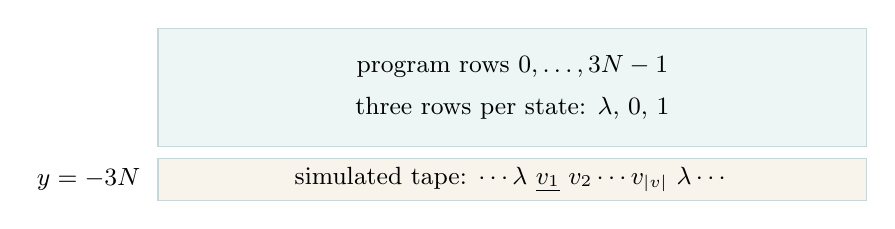
\begin{tikzpicture}[x=1cm,y=.6cm,font=\small]
\draw[fill=Pale,draw=Line] (0,0) rectangle (9,2.5);
\node at (4.5,1.7) {program rows $0,\ldots,3N-1$};
\node at (4.5,.8) {three rows per state: $\blank$, $0$, $1$};
\draw[fill=Warm,draw=Line] (0,-1.15) rectangle (9,-.25);
\node at (4.5,-.7) {simulated tape: $\cdots\blank\ \underline{v_1}\ v_2\cdots v_{|v|}\ \blank\cdots$};
\node[left] at (-.1,-.7) {$y=-3N$};
\end{tikzpicture}
\end{center}

\textbf{Rune Semantics.}
Each of $X,Y,Z$ has one position and a hidden symbol. Writing a rune first
restores the hidden symbol at the old rune position, then installs the rune over
the symbol at the new position. Rewriting a rune in place preserves the hidden symbol. Writing an ordinary symbol at a rune removes that rune.
A motion $X$, $Y$ or $Z$ jumps to the corresponding rune after the write.
Ordinary motions move one cell; $S$ stops without moving.

The \emph{logical program} means the program with every rune replaced by the corresponding hidden symbol. Correctness depends on preserving this logical program,
not on treating a rune as a destructive overwrite.

\newpage
\subsection{Endpoint and Prefix Invariant}\label{sec:part2}
\begin{lemma}[Endpoint and Prefix Invariant]\label{lem:geometry}
At the start of every simulated step, the expert occupies state $0$ at the
simulated tape head. Rune $X$ occupies column $1$ on the first or last row
of the current simulated state's three-row block. After matching $j$
successor trits, $X$ occupies column $1+j$ on a row with the correct
length-$j$ successor prefix. The row index remains congruent to $0$ or $2$
modulo $3$. The logical program remains unchanged.
\end{lemma}
\begin{proof}
Initially $X$ occupies the first row of state $0$. Assume the invariant at
the start of a simulated step. The expert reads the tape symbol, installs
$Z$, jumps to $X$, and steps left. The symbol search selects the matching
row within the current state's three-row block. The following right scan
crosses column $1$ and the source code to the first delimiter, leaving $X$
in place.

For successor trit $t$, the expert places $Y$ on the trit, jumps to $X$, and
steps right to the next source-code column. All rows sharing the matched
prefix form one interval. Within that interval, next-trit values increase
monotonically down the table. The successor state exists, so a nonempty
subinterval contains next trit $t$. Moving down on a smaller trit, or up
on a larger trit, reaches $t$ before leaving the matched-prefix interval.

An immediate match preserves the endpoint. A downward search enters the
target subinterval at the first row, with read symbol $\blank$; an upward
search enters at the last row, with read symbol $1$. Both rows occupy
endpoints of three-row state blocks. Writing $X$ advances the matched
prefix by one trit. Jumping to $Y$ resumes instruction decoding.

After all $\kappa$ trits, $X$ occupies a row in the successor state's block.
The second delimiter triggers a leftward rewind of $X$ to column $1$ on
the same row. The expert then applies the prescribed write and motion at
$Z$. Rune relocation restores every covered program symbol, preserving
the logical program. Each nonstopping motion establishes the next simulated step.
\end{proof}

\begin{lemma}[No Missing Middle Trit]\label{lem:middle}
Within a fixed source-code prefix block, a vertical search cannot pass
directly between an $L$ region and an $S$ region. A nonempty $R$ region
separates the two regions.
\end{lemma}
\begin{proof}
The state numbers fill the contiguous interval $0,\ldots,N-1$, with a common
encoding width. A prefix block contains a possibly truncated interval of
consecutive integers. A block containing next-trit values $L$ and $S$ also
contains every state in the intervening $R$ subinterval. Each state
contributes all three read-symbol rows.
\end{proof}

\begin{corollary}[Faithful Expert Simulation]\label{cor:simulation}
Each simulated TM transition takes finitely many controller steps and
performs the write and motion prescribed by $\delta$. The expert halts
exactly when the simulated TM issues $S$.
\end{corollary}
\begin{proof}
Lemma~\ref{lem:geometry} selects the correct instruction and successor.
Every scan stays within a finite program interval, and every trit search
reaches a nonempty target interval. The final two instruction fields supply
the prescribed write and motion at $Z$. Only a simulated $S$ triggers a
stopping transition.
\end{proof}

\clearpage
\sectiontitle{3 \enspace OBSERVATION PROTOCOL}{Observation Protocol}\label{sec:common3}
\label{sec:protocol}
The protocol records finite geometric context. Let $e\in\{0,2\}$ identify the endpoint row occupied by $X$.
Use $r,j\in\{0,1,2\}$ to index tape symbols and $t,a\in\{L,R,S\}$ to denote trits. A vertical search records the last
observed trit. Each phase and parameter tuple determines an expert state.

\begin{center}
\footnotesize\renewcommand{\arraystretch}{1.13}
\begin{tabularx}{\textwidth}{l c X}
\toprule\rowcolor{Pale}Phase & Expert state & Allowed reading and continuation\\\midrule
Initial & $0$ & Read $0$ or $1$; select the matching row from endpoint $0$.\\
Dispatch$(e)$ & $0$ & Read $\sigma_r$; jump to selection of $r$.\\
Selection jump$(e,r)$ & $1+r$ & Read $X$; step left to row index $j=e$.\\
Select$(e,r,j)$ & $1+r$ & Read $\sigma_j$; if $j=r$, cross column $1$; otherwise change $j$ by $\operatorname{sgn}(r-j)$.\\
Cross$(e,r)$ & $4$ & Read $X$ if $e=r$, and $\blank$ otherwise; enter first source trit.\\
First source trit$(e)$ & $4$ & Read any trit; enter remaining source-code scan.\\
Source scan$(e)$ & $4$ & Trit: repeat. Delimiter $0$: enter first successor trit.\\
First successor trit$(e)$ & $5$ & Read a trit $t$; jump to $X$ for matching $t$.\\
Successor scan$(e)$ & $5$ & Trit $t$: match $t$. Delimiter $0$: start rewind.\\
Match jump$(e,t)$ & $g_t$ & Read $X$; step right and begin comparison.\\
First comparison$(e,t)$ & $g_t$ & Read $a$. If $a=t$, resume with endpoint $e$; if $a<t$, search down; if $a>t$, search up.\\
Search down$(t,a)$ & $g_t$ & Read $a$ or the immediate successor of $a$. Repeat until $t$; then resume with endpoint $0$.\\
Search up$(t,a)$ & $g_t$ & Read $a$ or the immediate predecessor of $a$. Repeat until $t$; then resume with endpoint $2$.\\
Resume$(e,t)$ & $g_t$ & Read $Y$; advance to successor scan with endpoint $e$.\\
Rewind jump$(e)$ & $9$ & Read $X$; step left.\\
Rewind$(e)$ & $9$ & Trit: continue left. Blank: move $X$ here and jump to $Y$.\\
Rewind return$(e)$ & $9$ & Read $Y$; step right to the write field.\\
Read write$(e)$ & $10$ & Read $\sigma_r$; remember this write symbol.\\
Read motion$(e,r)$ & $11+r$ & Read $M\in\{L,R,S\}$; jump to $Z$.\\
Apply$(e,r,M)$ & $h_{r,M}$ & Read $Z$; write $\sigma_r$ and move $M$. Dispatch$(e)$ if $M\ne S$; otherwise halt.\\
Halt & $14$ & No outgoing action.\\
\bottomrule
\end{tabularx}
\end{center}
Here $g_L=6$, $g_R=7$, $g_S=8$, and
\[
h_{r,L}=1+2r,\qquad h_{r,R}=2+2r,\qquad h_{r,S}=11+r.
\]
The protocol starts at Initial; later simulated steps start at Dispatch$(e)$.
Searches update the remembered trit
after each change. Thus a downward search for $S$ that has seen $L$ must see
$R$ before $S$. The protocol permits unbounded repetition while retaining finite annotations.

\begin{lemma}[Protocol Coverage]\label{lem:coverage}
Every expert execution on a correct encoding with nonempty input follows
this protocol.
\end{lemma}
\begin{proof}
Initially the tape head reads $0$ or $1$, and $X$ occupies endpoint $0$.
Endpoint selection and the following column-$1$ reading follow from Lemma~\ref{lem:geometry}.
Both state codes have positive width. Prefix-block monotonicity and
Lemma~\ref{lem:middle} give the allowed vertical-search readings and endpoint
updates. Rewind reaches the blank in column $1$, then $Y$, the write field,
the motion field and $Z$. These exhaust the phases of one simulated step;
induction gives coverage for every finite prefix of the execution.
\end{proof}

The protocol permits additional observation sequences, including unequal
lengths for the two code scans. The certificate checks every permitted
transition, so this overapproximation preserves the equivalence argument.

\clearpage
\sectiontitle{4 \enspace SIMULATION CERTIFICATE}{Simulation Certificate}\label{sec:common4}
\subsection{Initial Entry, Row Selection and Code Scanning}\label{sec:part4}
For phase $i$, write $Q_i$ for the controller-state set specified in the
following certificate subsections. Relate configurations with identical grids, heads
and rune records, with expert state $g_i$ and controller state in $Q_i$.

\textbf{Initial and Subsequent Dispatches.}
The Initial phase has $Q_i=\{0\}$ and permits $0,1$ only, with successors
$1,35$, respectively. Dispatch$(e)$ has $Q_i=\{17\}$ for either endpoint
$e$, with successors $18,24,26$ on $\blank,0,1$. Every permitted transition
writes $Z$ and teleports to $X$, matching expert state $0$.
The certificate distinguishes the two initial selection routes.

\textbf{The Complete Row-Selection Routes.}
Each state list gives the controller state \emph{before each reading}; after
the final reading, the controller enters state $5$ at the first source-code
trit. The table represents each endpoint by the corresponding read symbol,
$\blank$ or $1$.

\begin{center}
\small\renewcommand{\arraystretch}{1.3}\setlength{\tabcolsep}{7pt}
\begin{tabular}{l c c l l}
\toprule\rowcolor{Pale}Entry & Endpoint & Wanted & Readings in order & States in order\\\midrule
Initial & $\blank$ & $0$ & $X,\blank,0,\blank$ & $1,2,3,4$\\
Initial & $\blank$ & $1$ & $X,\blank,0,1,\blank$ & $35,36,37,38,4$\\\midrule
Later & $\blank$ & $\blank$ & $X,\blank,X$ & $18,19,20$\\
Later & $\blank$ & $0$ & $X,\blank,0,\blank$ & $24,25,3,4$\\
Later & $\blank$ & $1$ & $X,\blank,0,1,\blank$ & $26,27,37,38,4$\\
Later & $1$ & $\blank$ & $X,1,0,\blank,\blank$ & $18,19,32,33,4$\\
Later & $1$ & $0$ & $X,1,0,\blank$ & $24,25,3,4$\\
Later & $1$ & $1$ & $X,1,X$ & $26,27,20$\\
\bottomrule
\end{tabular}
\end{center}
The expert uses state $1+r$ during selection of $\sigma_r$, then state
$4$ for the final column-$1$ reading. The $X$ step moves left; comparisons move up
or down toward the wanted symbol; the matching and crossing steps move
right. Every step preserves the read symbol. Substitution in the original tables
checks every route and successor state $5$.

Taking the union where Initial and Later routes share a phase gives exactly
the needed multivalued sets. For endpoint $0$ and wanted symbol $0$, the selection-jump and first-comparison sets equal $\{1,24\}$ and
$\{2,25\}$, respectively. For endpoint $0$ and wanted symbol $1$, the same
sets equal $\{26,35\}$ and $\{27,36\}$. Every other phase/parameter set
contains one controller state.

\textbf{Source and Successor Code Scans.}
The first and subsequent source-trit phases both have $Q_i=\{5\}$.
State $5$ preserves each trit, moves right, and remains $5$.
On delimiter $0$, state $5$ preserves $0$, moves right, and enters state $6$.
Both the first successor-trit phase and the subsequent successor scan
have $Q_i=\{6\}$, with the following transitions:
\begin{center}
\small\renewcommand{\arraystretch}{1.3}
\begin{tabular}{c cccc}
\toprule\rowcolor{Pale}Controller state & Read $L$ & Read $R$ & Read $S$ & Read $0$\\\midrule
$6$ & $7$ & $10$ & $28$ & $11$\\
\bottomrule
\end{tabular}
\end{center}
Entries list successor states; each action writes $Y$ and teleports to $X$.
The delimiter branch follows at least one successor trit.
Expert state $5$ enters $6,7,8$ for trits $L,R,S$, and $9$ for the delimiter.
This gives the match-jump states $7,10,28$ and rewind-jump state $11$.

\newpage
\subsection{Matching Trits, Rewinding and Updating the Tape}\label{sec:part5}
\textbf{Match One Successor Trit.}
The match-jump states $7,10,28$ preserve $X$, move right and enter $8,10,29$,
respectively, for targets $L,R,S$. The following table gives the comparison actions.

\begin{center}
\small\renewcommand{\arraystretch}{1.35}
\begin{tabular}{c c ccc}
\toprule\rowcolor{Pale}Target & State & Read $L$ & Read $R$ & Read $S$\\\midrule
$L$ & $8$ & $\triple{9}{X}{Y}$ & $\triple{8}{R}{U}$ & $\triple{8}{S}{U}$\\
$R$ & $10$ & $\triple{10}{L}{D}$ & $\triple{9}{X}{Y}$ & $\triple{10}{S}{U}$\\
$S$ & $29$ & $\triple{29}{L}{D}$ & $\triple{29}{R}{D}$ & $\triple{9}{X}{Y}$\\
\bottomrule
\end{tabular}
\end{center}
These rows cover every permitted first-comparison and vertical-search
phase, paired with expert states $6,7,8$.
On a match, writing $X$ advances the bookmark and teleporting to $Y$
returns to the instruction. Resume$(e,t)$ has $Q_i=\{9\}$ for every endpoint
and target: state $9$ preserves $Y$, moves right, and enters state $6$.

\textbf{Rewind $X$ and Reach the Write Field.}
All rewind phases use expert state $9$ and follow this sequence:
\begin{center}
\small\renewcommand{\arraystretch}{1.3}
\begin{tabular}{l c c l}
\toprule\rowcolor{Pale}Phase & Controller state & Reading & Transition\\\midrule
Rewind jump & $11$ & $X$ & $\triple{12}{X}{L}$\\
Rewind through code & $12$ & $t\in\{L,R,S\}$ & $\triple{12}{t}{L}$\\
Rewind reaches column $1$ & $12$ & $\blank$ & $\triple{13}{X}{Y}$\\
Rewind return & $13$ & $Y$ & $\triple{14}{Y}{R}$\\
\bottomrule
\end{tabular}
\end{center}
The final step enters expert state $10$, so ReadWrite$(e)$ has $Q_i=\{14\}$.
On reading $\blank,0,1$, state $14$ preserves that symbol, moves right and
enters $15,21,30$, respectively. The corresponding expert transitions enter states $11,12,13$.

\textbf{Motion Decoding and Tape Update.}
Each motion-reading transition writes $Y$, teleports to $Z$, and enters
the apply state below. That state reads $Z$, writes the row's symbol and
performs exactly the chosen motion.
\begin{center}
\small\renewcommand{\arraystretch}{1.35}\setlength{\tabcolsep}{10pt}
\begin{tabular}{c c ccc}
\toprule\rowcolor{Pale}Write symbol & Motion-reading state & Apply $L$ & Apply $R$ & Apply $S$\\\midrule
$\blank$ & $15$ & $16$ & $23$ & $34$\\
$0$ & $21$ & $40$ & $22$ & $42$\\
$1$ & $30$ & $39$ & $31$ & $41$\\
\bottomrule
\end{tabular}
\end{center}
The $L$ and $R$ apply transitions return to controller state $17$, paired
with expert state $0$ in Dispatch$(e)$. Either motion may reach a blank tape cell;
state $17$ handles that case correctly. The $S$ transitions enter controller
halt state $43$, paired with expert halt state $14$.

\textbf{Certificate Size.}
These certificate subsections specify every $Q_i$, including the four doubletons caused
by initial versus later selection. The $92$ reachable parameterized phases
produce $96$ related phase--state pairs. The $160$ local checks cover
all $73$ defined nonterminal entries of the exported controller.
The remaining nine defined entries contain halt loops, excluded from
PTOs. Every permitted successor belongs to the next phase's controller-state set.

For each permitted protocol edge $i\xrightarrow{x}j$ and each $q\in Q_i$,
the preceding certificate establishes
\begin{equation}
\delta_\EXPERT(g_i,x)=(g_j,w,M),\qquad
\delta_\CTRL(q,x)=(q',w,M),\qquad q'\in Q_j. \tag{2}
\end{equation}
Every required entry exists. A transition reaches a halt state exactly
on an edge to the terminal phase, with motion $S$.

\clearpage
\sectiontitle{5 \enspace EQUIVALENCE PROOF}{Equivalence Proof}\label{sec:common5}
\label{sec:equivalence}
\begin{proof}[Proof of Theorem~\ref{thm:main}]
Initially both configurations have the same grid, head, and rune records,
with control states $0$ related by Initial. Suppose the relation holds
before a controller step. Lemma~\ref{lem:coverage} supplies an allowed read symbol
$x$. Equal grids and heads give the same read symbol to both controllers.
Equation~(2) gives equal writes and motions and preserves the relation
between successor states. The next grids and heads therefore agree.
Rune installation, restoration, and teleportation act deterministically,
so the rune records also agree.

Induction establishes equality of every finite execution prefix. The terminal
condition permits a halt exactly on an edge to the terminal phase.
Consequently, both controllers halt on the same step or both execute
infinitely many steps with equal finite prefixes. Corollary~\ref{cor:simulation}
identifies the expert execution with the encoded TM computation.
\end{proof}

\textbf{Counterexample to the Claim Including Empty Input.}
Use a one-state TM that preserves the read symbol and immediately stops:
\[
\delta(0,s)=(0,s,S)\qquad\text{for every }s\in\{\blank,0,1\},
\]
and input $v=\varepsilon$. This pair satisfies the encoder's total-TM
contract. With one-trit state code $L$, the encoded program contains:
\begin{center}
\small\renewcommand{\arraystretch}{1.25}
\begin{tabular}{c cccccccc}
\toprule\rowcolor{Pale}Row & Read & Bookmark & State & Delim. & Next & Delim. & Write & Move\\\midrule
$0$ & $\blank$ & $X$ & $L$ & $0$ & $L$ & $0$ & $\blank$ & $S$\\
$1$ & $0$ & $\blank$ & $L$ & $0$ & $L$ & $0$ & $0$ & $S$\\
$2$ & $1$ & $\blank$ & $L$ & $0$ & $L$ & $0$ & $1$ & $S$\\
\bottomrule
\end{tabular}
\end{center}
The tape contains only blanks, and the head starts at $(1,-3)$.
The expert takes transition $\delta_\EXPERT(0,\blank)=\triple{1}{Z}{X}$,
producing first PTO triple $(\blank,Z,X)$. The controller lacks the entry
$\delta_\CTRL(0,\blank)$ and cannot produce that triple. Thus the unrestricted equivalence claim
fails at the \emph{first} controller step; the expert continues and halts
after $17$ steps. The file \path{empty_input_counterexample.json} records the witness and full expert PTO.

\clearpage
\sectiontitle{6 \enspace VERIFICATION AND ARTIFACTS}{Verification and Artifacts}\label{sec:common6}
Run
\begin{center}\code{python3 verify\_equivalence.py {-}{-}quick}\end{center}
from this proof directory. The checker uses only the Python standard library and checks
source fingerprints, CSV/JSON agreement, the exported expert against
\code{universal\_tp}, all $160$ obligations of the nonempty-input certificate,
and coverage of all $73$ defined nonterminal entries. The checker also reconstructs
the empty-input counterexample without modifying a controller file.

\textbf{Independent Complete Executions and Finite Prefixes.}
Omitting \code{{-}{-}quick} additionally compares two independent grid memories
with separate heads and rune records. The checker compares the decoded instruction
against a direct simulated TM at each completed simulated step, including
the tape, current state and head, and preservation of the logical program.

The suite includes every one-state total transition table ($729$ choices)
on every nonempty input word of lengths $1$--$3$ ($14$ words), giving
$10{,}206$ exhaustive cases. The suite also includes $128$ fixed-seed random cases
and $42$ directed cases around ternary-width boundaries. Programs have up
to $2{,}188$ states and eight-trit state encodings.

All $1{,}067{,}993$ controller transitions agree across
$42{,}557$ simulated TM steps. The execution checks exercise every defined nonterminal entry. Of the $10{,}376$ cases, $6{,}509$ halt within the
simulation limit, and $3{,}867$ contribute finite prefixes. Bounded runs
establish no eventual-halting or nonhalting conclusion; induction proves
the infinite-execution theorem.

\textbf{Printed-Table Verification.}
Printed-table verification compares all $396$ cells of the two-page PDF
against the CSV: $82$ defined entries and $314$ undefined cells. This includes the
missing blank entry in initial state $0$. With \code{pypdf} installed,
\code{python3 verify\_equivalence.py {-}{-}quick {-}{-}check-pdf} repeats the check.

\textbf{Artifact Identity.}
The title page gives the repository-relative case directory. This proof directory
contains the controller and expert exports, reference code, protocol, checker,
and saved verification report. The verification script stores or reads SHA-256 checksums for these artifacts. A checksum identifies the exact bytes
of a file; the checker compares the stored and computed values to detect changes.
These checks bind the certificate to the supplied exports. The invariants,
protocol coverage, and local transition identity establish equivalence.
\end{document}
